\chapter{Metodología}

En este capítulo vamos a definir y a detallar las herramientas necesarias y los procesos que vamos a seguir para solucionar el problema planteado en base a los objetivos que presentamos en el segundo capítulo y a los antecedentes vistos en el tercero.

\section{Herramientas utilizadas}

\subsection{OWASP ZAP}

Analizar la seguridad es una tarea compleja que requiere tener en cuenta multitud de factores por lo que realizar dicho análisis de forma manual resulta poco menos que imposible. Por ello vamos a utilizar \texttt{ZAP} que es un analizador de vulnerabilidades de código abierto desarrollado por la organización \texttt{OWASP}. Dicho analizador fue una de las herramientas que obtuvo el premio \textit{Bossie 2015} al mejor software de red y seguridad de código abierto \cite{staff_bossie_2015}.

\bigskip
Aunque ZAP tiene una interfaz gráfica (ver \ref{fig:owasp_zap}) para nuestro proyecto vamos a automatizar su uso mediante la API disponible en lenguaje Python.


\begin{figure}[H]
\centering
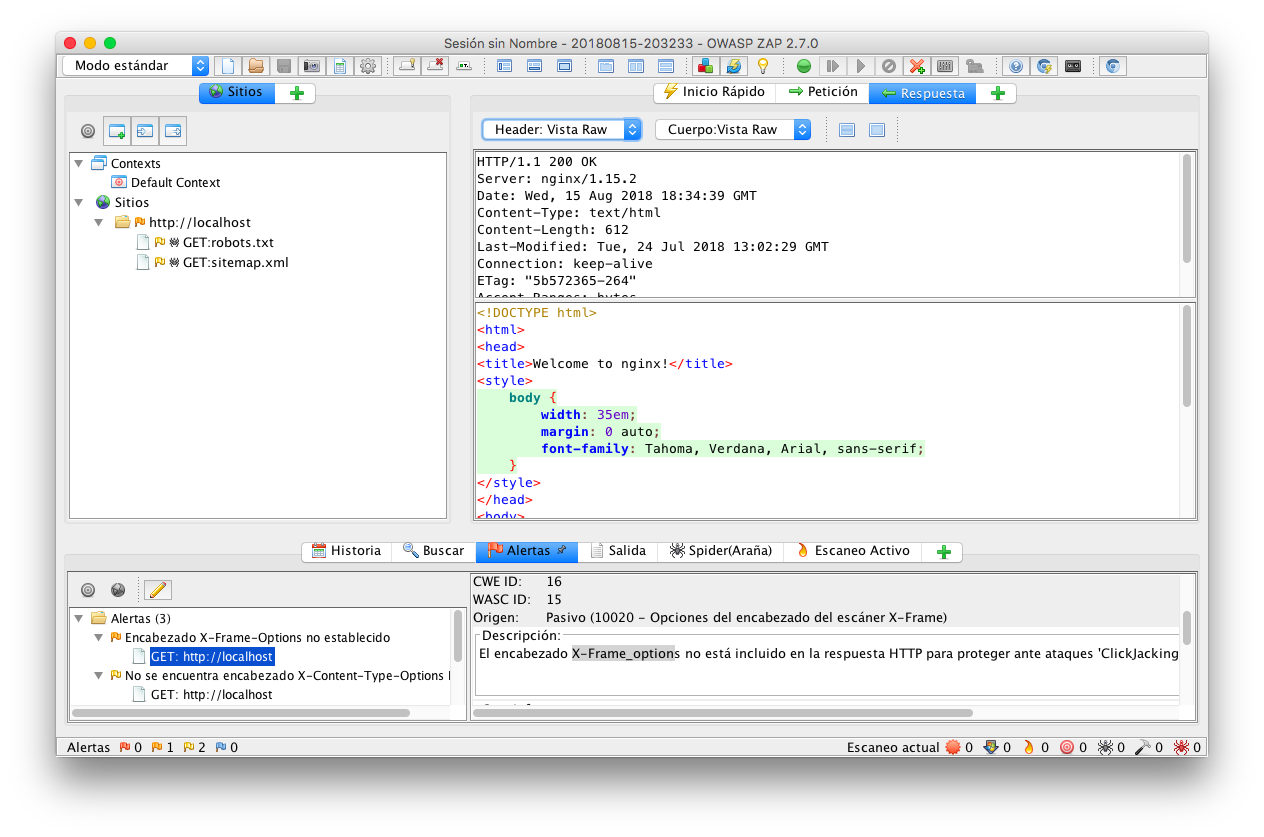
\includegraphics[width=1.0\textwidth]{../images/owasp-zap-main-window}
\caption{Ventana principal de OWASP ZAP}
\label{fig:owasp_zap}
\end{figure}


\subsection{Docker}
Para simular diferentes servidores de una forma rápida se ha optado por usar un sistema de virtualización ligera basada en contenedores. Para esto se ha usado \textbf{Docker} que es uno de los sistemas de virtualización ligera basada en contenedores más utilizada. Para la orquestación de los diferentes contenedores (Servidor y Analizador) se utilizará el estándar \textbf{docker-compose} que nos permite definir un conjunto de contenedores de una forma sencilla en un fichero de texto YML.

\bigskip
La orquestación estará compuesta de dos contenedores, uno basado en \textit{Alpine Linux} en el que instalaremos el servidor que vayamos a analizar y un segundo contenedor basado en la imagen oficial de ZAP que podemos encontrar en la URL: \url{https://hub.docker.com/r/owasp/zap2docker-bare/}.

\subsection{Python}

Se ha decidido desarrollar este proyecto en el lenguaje de programación Python debido a estar familiarizado con este lenguaje y a la disponibilidad de una API de OWASP ZAP en dicho lenguaje. Además, aunque este proyecto no requiere un elevado rendimiento, diversas publicaciones indican un muy buen desempeño del lenguaje Python a la hora de trabajar con algoritmos genéticos \cite{merelo-guervos_comparison_2016}.

\bigskip
Se han seguido buenas práctias de programación como pueden ser escribir pruebas unitarias de cada función desarollada. Para ejecutar dichas pruebas unitarias se ha utilizado la herramienta \texttt{pytest}. También se ha tenido en cuenta que la codificación siga una guía de estilo, concretamente \texttt{PEP8} que son es la guía de estilo considerada `oficial' por parte de los desarrolladores de Python.

\section{Análisis general del problema}

Teniendo en cuenta la ingente cantidad de servicios de red con sus múltiples opciones de configuración se ha optado por limitar este proyecto a alterar y optimizar la configuración de un servidor HTTP, concretamente NGINX ya en los últimos años ha desbancado a Apache como el servidor HTTP  más utilizado del mundo \cite{w3techs_usage_2019}.

\bigskip
La elección del protocolo HTTP ha sido porque es el protocolo de capa de aplicación más extendido y utilizado en Internet, de hecho el estudio `Global Internet Phenomena Report' de 2018 sitúa a HTTP muy por encima de otros servicios como la VoIP, la mensajería y los servicios de juegos en línea \cite{sandvine_2018_2018}.

\bigskip
La configuración de NGINX, al igual que la de muchos otros servidores, se realiza mediante ficheros de texto plano con una sintaxis específica, la misma se puede encontrar definida en la siguiente URL: \url{http://nginx.org/en/docs/beginners_guide.html#conf_structure} y consta de múltiples directivas, podemos ver un ejemplo aquí: \ref{lst:nginx_config}.

Como podemos observar un fichero de configuración de NGINX tiene diferentes directivas que se pueden configurar de diferentes maneras, tanto para optimizar como para simplemente simular una configuración distinta y así hacer creer a un atacante que hemos cambiado de servidor HTTTP o incluso de servidor físico.

\section{Banco de pruebas}

Para empezar definimos un banco de pruebas para comprobar que la herramienta OWASP ZAP servía para nuestro propósito. Para ello se modificó el código de ejemplo que proporcionan para su API en Python para hacerla funcionar en un entorno de contenedores. El script (zap.py \ref{zap.py}) se conecta a una determinada URL y ejecuta una serie de comprobaciones para terminar devolviendo el número de vulnerabilidades encontradas. Dichas vulnerabilidades están basadas en la escala CVSS por lo que hay vulnerabilidades consideradas críticas y otras que son solo sugerencias.

\bigskip
A la hora de obtener una web para testear se estuvo barajando el uso de diferentes entornos web como pueden ser Galileo (Perl), WordPress (PHP), una simple web realizada en html\ref{lst:simple_html_web} e incluso una aplicación web premeditadamente vulnerable desarrollada por OWASP llamada \texttt{Juice-Shop} realizada con \textbf{Node.js} pero al final se optó por utilizar el mensaje de bienvenida de `NGINX' (ver \ref{lst:nginx_welcome_message}). La configuración estándar de NGINX con dicho mensaje nos mostraba 5 alertas \ref{lst:owas_zap_welcome_message_alerts} siendo mucho mas fácil de gestionar que las 71 que obteníamos con ``Juice-Shop''.

\bigskip
Una parte muy importante para el correcto funcionamiento de OWASP ZAP fue simular un dominio, en este caso utilizamos el conocido \textbf{example.com} que es un nombre reservado por la IANA (Internet Assigned Numbers Authority) en el RFC2606 \cite{eastlake_reserved_1999}. Para hacer uso del mismo se ha optado por darle ese nombre de \textbf{host} al contenedor que levanta NGINX.

\bigskip
Una vez hemos generado nuestro laboratorio para pruebas y viendo que se NGINX se ejecuta correctamente pasamos a probar como va cambiando la respuestas de OWASP ZAP dependiendo de la configuración de nuestro NGINX. Para ello agregamos la cabecera \begin{verbatim}add_header X-Frame-Options "SAMEORIGIN";\end{verbatim} y ejecutamos el conjunto, dándonos 4 vulnerabilidades en lugar de las 5 anteriores. Esta prueba nos indica que efectivamente la modificación de los parámetros de NGINX puede darnos configuraciones más o menos seguras.

\section{Eligiendo los parámetros}

La última versión de NGINX (1.17.2) posee 739 directivas de configuración por lo que para simplificar nuestra tarea vamos a limitarnos a un conjunto mas pequeño de directivas (ver tabla \ref{table:apache_nginx_directives}).

\bigskip
En un primer momento pensamos en basarnos en las directivas \textbf{STIG}, pero estas directivas sólo están definidas para el servidor Apache. Por suerte al ser HTTP un estándar muchas de las directivas de Apache tienen su símil en NGINX por lo que hemos extraído un conjunto de las mas representativas y que además tuvieran su equivalente para el servidor NGINX. Las puntuaciones se basan en el sistema de puntuación CVSS de acuerdo con los resultados devueltos por ZAP con el código de prueba. También se han agregado algunas cabeceras identificativas como pueden ser la identificación del servidor (ver tabla \ref{table:ngingx_headers}) así como la directivas de compresión \texttt{gzip} para tener una mayor entropía.

\begin{table}[H]
\begin{tabular}{|l|l|l|l|}
\hline
Id & STIG ID & Configuración Apache  & Equivalente NGINX              \\ \hline
0  & V-13730 & MaxClients            & worker\_connections            \\ \hline
1  & V-13726 & KeepAliveTimeout      & keepalive\_timeout             \\ \hline
2  & V-13732 & FollowSymLinks        & disable\_symlinks              \\ \hline
3  & V-13735 & Indexes               & autoindex                      \\ \hline
4  & V-13724 & Timeout               & send\_timeout                  \\ \hline
5  & V-13738 & LimitRequestFieldsize & large\_client\_header\_buffers \\ \hline
6  & V-13736 & LimitRequestBody      & client\_max\_body\_size        \\ \hline
7  & V-6724  & ServerTokens          & server\_tokens                 \\ \hline
8  &         &                       & gzip                           \\ \hline
\end{tabular}
\label{table:apache_nginx_directives}
\caption{Lista de directivas NGINX utilizadas}
\end{table}

\begin{table}[H]
\begin{tabular}{|l|l|}
\hline
Id & Cabecera                       \\ \hline
9  & X-Frame-Options                \\ \hline
10  & X-Powered-By                   \\ \hline
11 & X-Content-Type-Options         \\ \hline
12 & Server                         \\ \hline
\end{tabular}
\label{table:ngingx_headers}
\caption{Lista de cabeceras HTTP utilizadas}
\end{table}


\bigskip
Pasamos a detallar que realiza cada directiva escogida y sus posibles valores:

\subsection{worker\_connections}

\begin{table}[H]
\begin{tabular}{|l|l|}
\hline
Sintaxis      & worker\_connections number; \\ \hline
Por defecto   & worker\_connections 512;     \\ \hline
Contexto      & events     \\ \hline
\end{tabular}
\end{table}

Establece el número máximo de conexiones simultáneas que pueden ser abiertas por un proceso de NGINX.

\bigskip
Debe tenerse en cuenta que este número incluye todas las conexiones (por ejemplo, conexiones con servidores proxy, entre otros), no sólo las conexiones con clientes. Otra consideración es que el número real de conexiones simultáneas no puede exceder el límite actual del número máximo de archivos abiertos.

\subsection{keepalive\_timeout}

\begin{table}[H]
\begin{tabular}{|l|l|}
\hline
Sintaxis      & keepalive\_timeout timeout; \\ \hline
Por defecto   & keepalive\_timeout 75s;     \\ \hline
Contexto      & http, server, location     \\ \hline
\end{tabular}
\end{table}

Establece un tiempo de espera durante el cual una conexión cliente permanecerá abierta en el lado del servidor. El valor cero deshabilita las conexiones de cliente Keep-alive. La cabecera ``Keep-Alive: timeout=time'' está soportada por Firefox y Chrome. Internet Explorer cierra las conexiones abiertas por sí mismo en unos 60 segundos.

\subsection{disable\_symlinks}

\begin{table}[H]
\begin{tabular}{|l|l|}
\hline
Sintaxis      & disable\_symlinks on \textbar  off; \\ \hline
Por defecto   & disable\_symlinks off;     \\ \hline
Contexto      & http, server, location     \\ \hline
\end{tabular}
\end{table}

Determina cómo se deben tratar los enlaces simbólicos al abrir archivos. Cuando está desactivado los enlaces simbólicos en la ruta de acceso están permitidos y no están marcados. Este es el comportamiento por defecto. Cuando está activado y algún componente de la ruta de acceso es un enlace simbólico, se deniega el acceso a ese archivo.

\subsection{autoindex}

\begin{table}[H]
\begin{tabular}{|l|l|}
\hline
Sintaxis      & autoindex on \textbar  off; \\ \hline
Por defecto   & autoindex off;     \\ \hline
Contexto      & http, server, location     \\ \hline
\end{tabular}
\end{table}

Cuando está activado muestra el contenido de los directorios, en caso contrario no muestra nada.

\subsection{send\_timeout}

\begin{table}[H]
\begin{tabular}{|l|l|}
\hline
Sintaxis      & send\_timeout time; \\ \hline
Por defecto   & send\_timeout 60s;     \\ \hline
Contexto      & http, server, location     \\ \hline
\end{tabular}
\end{table}

Establece el tiempo de espera para transmitir una respuesta al cliente. El tiempo de espera se establece sólo entre dos operaciones de escritura sucesivas, no para la transmisión de la respuesta completa. Si el cliente no recibe nada en este tiempo, la conexión se cierra.

\subsection{large\_client\_header\_buffers}

\begin{table}[H]
\begin{tabular}{|l|l|}
\hline
Sintaxis      & large\_client\_header\_buffers number size; \\ \hline
Por defecto   & large\_client\_header\_buffers 4 8k;     \\ \hline
Contexto      & http, server     \\ \hline
\end{tabular}
\end{table}

Establece el número máximo y el tamaño de los búferes utilizados para leer los encabezados de solicitudes de clientes grandes. Una línea de petición no puede exceder el tamaño de un búfer, o el error 414 (Request-URI Too Large) es devuelto al cliente. Un campo de encabezado de solicitud no puede exceder el tamaño de un búfer también, o el error 400 (Bad Request) es devuelto al cliente. Los búferes se asignan sólo bajo demanda. Por defecto, el tamaño del búfer es igual a 8K bytes. Si una vez finalizada la tramitación de la solicitud, la conexión pasa al estado de espera, se liberan estos búferes.

\subsection{client\_max\_body\_size}

\begin{table}[H]
\begin{tabular}{|l|l|}
\hline
Sintaxis      & client\_max\_body\_size size; \\ \hline
Por defecto   & client\_max\_body\_size 1m;     \\ \hline
Contexto      & http, server, location     \\ \hline
\end{tabular}
\end{table}

Establece el tamaño máximo permitido del cuerpo de la solicitud del cliente, especificado en el campo ``Content-Length'' del encabezado de la solicitud. Si el tamaño de una solicitud excede el valor configurado, el error 413 (Request Entity Too Large) se devuelve al cliente. Tenga en cuenta que los navegadores no pueden mostrar correctamente este error. Configurar el tamaño a 0 desactiva la comprobación del tamaño del cuerpo de la solicitud del cliente.

\subsection{server\_tokens}

\begin{table}[H]
\begin{tabular}{|l|l|}
\hline
Sintaxis      & server\_tokens on \textbar  off; \\ \hline
Por defecto   & server\_tokens on;     \\ \hline
Contexto      & http, server, location     \\ \hline
\end{tabular}
\end{table}

Habilita o deshabilita la emisión de la versión NGINX en las páginas de error y en el campo ``Server'' del encabezado de respuesta.

\subsection{gzip}

\begin{table}[H]
\begin{tabular}{|l|l|}
\hline
Sintaxis      & gzip on \textbar  off; \\ \hline
Por defecto   & gzip off;     \\ \hline
Contexto      & http, server, location     \\ \hline
\end{tabular}
\end{table}

Habilita o deshabilita la compresión de las respuestas HTTP.

\subsection{X-Frame-Options}

\begin{table}[H]
\begin{tabular}{|l|l|}
\hline
Sintaxis      & X-Frame-Options: DENY \textbar  SAMEORIGIN \textbar  ALLOW-FROM url; \\ \hline
Contexto      & server, location     \\ \hline
\end{tabular}
\end{table}

La cabecera ``X-Frame-Options'' puede ser usada para indicar si debería permitírsele a un navegador renderizar una página de forma embebida . Las páginas web pueden usarlo para evitar ataques de \textit{clickjacking}, asegurándose que su contenido no es embebido en otros sitios.

\subsection{X-Powered-By}

\begin{table}[H]
\begin{tabular}{|l|l|}
\hline
Sintaxis      & X-Powered-by: NGINX; \\ \hline
Contexto      & server, location     \\ \hline
\end{tabular}
\end{table}

La cabecera ``X-Powered-By'' se usa para especificar con que software se ha generado la respuesta por parte del servidor.

\bigskip
Se recomienda no dar información demasiado extensa en dicha cabecera ya que puede revelar detalles que pueden facilitar la tarea de encontrar y explotar fallos de seguridad.


\subsection{X-Content-Type-Options}

\begin{table}[H]
\begin{tabular}{|l|l|}
\hline
Sintaxis      & X-Content-Type-Options: nosniff; \\ \hline
Contexto      & server, location     \\ \hline
\end{tabular}
\end{table}

El encabezado HTTP de respuesta ``X-Content-Type-Options'' es un marcador utilizado por el servidor para indicar que los tipos \textit{MIME} anunciados en los encabezados ``Content-Type'' no se deben cambiar ni seguir. Esto permite desactivar el ``MIME type sniffing''.

\bigskip
Introducido por Microsoft en Internet Explorer 8 e implementado paulatinamente por el resto de navegadores, ayuda a los administradores puedan bloquear el rastreo de contenido, pudiendo transformar tipos MIME no ejecutables en tipos MIME ejecutables.

\subsection{server}

\begin{table}[H]
\begin{tabular}{|l|l|}
\hline
Sintaxis      & Server: NGINX 1.12; \\ \hline
Contexto      & server, location     \\ \hline
\end{tabular}
\end{table}

La cabecera `Server' contiene la información acerca del software usado por el servidor.

\bigskip
Al igual que con la cabecera `X-Powered-By', se recomienda no dar información demasiado extensa en dicha cabecera ya que puede revelar detalles que pueden facilitar la tarea de encontrar y explotar fallos de seguridad.

\section{Metodología de desarrollo}

Utilizar una metodología como puede ser el desarrollo `en cascada` no es viable en un proyecto de estas características, ya que se ha ido aprendiendo como funcionaban diversas herramientas a la vez que se estaba escribiendo el código, porque lo que han habido multitud de cambios.

\bigskip
Para el desarrollo de nuestro sistema se ha optado por una metodología ágil. Concretamente nos hemos basado en la metodología `eXtreme Programming' o programación extrema. De hecho el carácter de investigación de este proyecto se amolda perfectamente a las directrices de esta metodología puesto que el software y los requisitos se han ido cambiando a medida que se iban obteniendo resultados con las distintas herramientas. 

\section{Diseño de la herramienta}

Para diseñar la herramienta hemos usado, como hemos mencionado anteriormente, el lenguaje de programación Python. Se han hecho uso de las librerías de código abierto \texttt{nginx-config-builder}, \texttt{ZAP API} así como \texttt{mock} para simular el comportamiento de funciones internas para conseguir una ejecución determinística de las pruebas unitarias.

\bigskip
La herramientas se compone de un sencillo \textit{script} `genetic.py' que es el algoritmo genético en sí y que hace uso de algunas funciones auxiliares tambien definidas por nosotros para calcular el `fitness' usando el valor numérico devuelto por ZAP así como para la generación de la configuración de NGINX y la generación de los individuos, en la figura \ref{fig:diagrama_1} se puede ver el diagrama de clases de nuestra herramienta con sus funciones definidas y en la figura \ref{fig:diagrama_2} podemos ver un diagrama de paquetes en los que se puede apreciar como funciona el conjunto de la aplicación en conjunto con el servidor NGINX y la herramienta OWASP ZAP.

\begin{figure}[H]
\centering
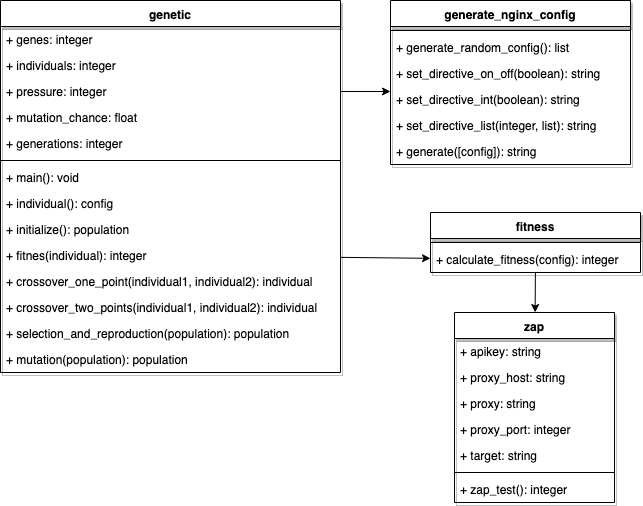
\includegraphics[width=1.0\textwidth]{../images/diagrama_1}
\caption{Diagrama de clases}
\label{fig:diagrama_1}
\end{figure}

\begin{figure}[H]
\centering
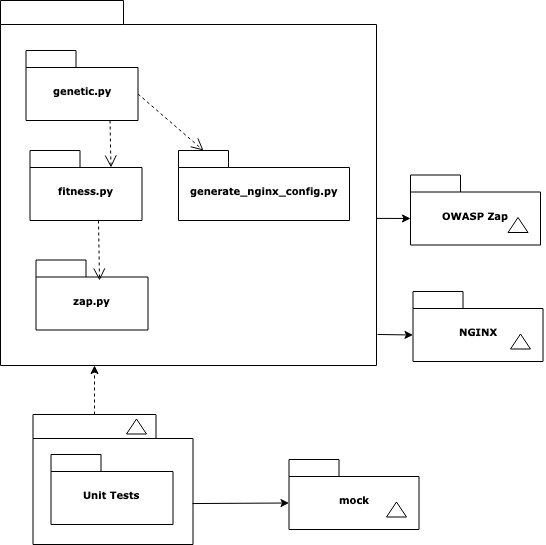
\includegraphics[width=1.0\textwidth]{../images/diagrama_2}
\caption{Diagrama de paquetes}
\label{fig:diagrama_2}
\end{figure}

En los siguientes puntos se detallará el desarrollo de cada una de las partes de la aplicación:

\subsection{Generación de configuraciones}

\bigskip
Para generar las distintas configuraciones de NGINX utilizamos la librería \textbf{nginx-config-builder} desarrollada por la empresa Linkedin y licenciada bajo la BSD. Dicha librería la podemos encontrar en \url{https://github.com/linkedin/nginx-config-builder}. Haciendo uso de esta librería desarrollamos un script \ref{generate_nginx_config.py} que en base a un cromosoma generaba una configuración, sin saber todavía si dicha configuración podía funcionar o no.

\bigskip
El siguiente paso es conseguir saber primeramente si la configuración funciona y después saber si la misma configuración funcional es segura. Para lo primero el propio NGINX tiene una herramienta de comprobación de configuración, la podemos invocar con el comando \textbf{NGINX -t <archivo-configuracion.conf>}, dicha herramienta nos comprueba que la sintaxis del fichero de configuración sea correcto y NGINX pueda ejecutarse sin problemas. Para lo segundo configuraremos un servidor NGINX con dicha configuración y haremos uso de la herramienta ZAP, para poder hacerlo de forma dinámica y sencilla utilizaremos la potencia de Docker.

\bigskip
Nuestra función de evaluación utilizará una combinación de estas dos herramientas, ya que el primero nos servirá para descartar directamente las configuraciones erróneas y la segunda nos permitirá establecer la calidad de una configuración con un valor escalar.

\subsection{Implementación del algoritmo genético}

La implementación del algoritmo genético utiliza una combinación de procesos de selección, cruzamiento y mutación para mejorar la solución a través de varias generaciones.

\bigskip
El algoritmo genético responderá al segundo objetivo `comprobar si utilizar una heurística de búsqueda, como pueden ser los algoritmos genéticos, puede servir para incrementar la seguridad de un sistema a la hora de generar configuraciones' 

\bigskip
Aunque en un primero momento se planteó el uso de algún `framework' de algoritmos genéticos como puede ser \textbf{DEAP}, desarrollado en Python, pero se optó en su lugar por utilizar un algoritmo sencillo que cubría de sobra nuestras necesidades.

\bigskip
Para la realización del algoritmo genético hemos utilizado como base uno de los múltiples ejemplos que hay en Internet. Concretamente el del estupendo tutorial que podemos encontrar en la web \textbf{robologs.net} concretamente en esta URL: \url{https://robologs.net/2015/09/01/}.

\bigskip
El sistema está diseñado para lograr el objetivo del planteamiento del problema. En este diseño, se han desarrollado dos algoritmos de cruzamiento (\textit{crossover}), uno donde cruza a dos individuos mediante un sólo punto de cruce y otro donde se utilizan dos puntos de cruce. 

\bigskip
El algoritmo genético se encarga de llamar a los anteriores \texttt{scripts} para generar soluciones de seguridad. En primer lugar, inicializa las soluciones aleatorias, que luego pasan por los procesos de selección, que se describen en detalle más adelante en este capítulo. El algoritmo genético depende de la puntuación de aptitud de cada solución para ir más allá en el proceso de selección, lo que significa que es responsabilidad del algoritmo de puntuación de aptitud dar puntuaciones para las soluciones y enviarlas más allá del algoritmo genético.

\bigskip
El algoritmo de puntuación (fitness.py \ref{fitness.py}) será el responsable de proporcionar al algoritmo genético las puntuaciones de fitness de las soluciones de seguridad. El sistema de puntuación se basa en las preferencias previas de STIG, que proporciona las vulnerabilidades, que será devuelto como un valor escalar dado por ZAP. Este valor escalar será un entero que puede ir de 0 a 999, siendo 0 una configuración sin ninguna vulnerabilidad y 999 una configuración incorrecta.

\bigskip
Básicamente el algoritmo crea una población de `n' individuos aleatorios definidos en la variable `individuals', y durante `i' generaciones, definidas en la variable `generations', los va seleccionado, cruzando y mutando. Para seleccionarlos lo que hace es otorgar una puntuación escalar con el algoritmo de fitness y ordenar la población de forma inversa, dejando al final de la lista los valores con menor fitness, pues son los que menor número de vulnerabilidades ha dado ZAP. Entonces se sustituyen los primeros elementos de la lista por el cruce de dos individuos aleatorios situados entre el final y el indicado por el valor `pressure' que siempre deberá ser al menos mayor que 2 para darle mayor diversidad. Entonces se mutan los elementos con una probabilidad definida en la variable `mutation\_chance' y se vuelve a lanzar el algoritmo hasta que no queden generaciones. Al finalizar el algoritmo seleccionaremos el último elemento de la lista de la población evolucionada como el mejor de todos.


